%% Diese Vorlage wurde am 24.08.2021 von Teresa Seidl Fernández erstellt 
%% und wird den Studenten/-innen der Fakultät für Angewandte Psychologie
%% der SRH Hochschule zur Verfügung gestellt und kann auch von ihnen
%% angepasst werden.






%%%%%%%%%%%%%%%%%%%%%%%%%%%% VORSPANN %%%%%%%%%%%%%%%%%%%%%%%%%

\documentclass[12pt, a4paper]{report}

\usepackage{SRH_Vorlage}

\usepackage[ngerman]{babel}        % n steht für neu und richtet sich an den
% neuen Rechtschreibregeln. Weitere Sprachen können verwendet werden. Um eine
% dieser Sprachen als "Hauptsprache" zu determinieren: main=[gewünschte Sprache]
\usepackage{ifthen}     % The package’s basic command is \ifthenelse, which 
% can use a wide array of tests. Also provided is a simple loop command 
% \whiledo. Ifthen is a separate package within the LaTeX distribution; 
% while it will always be present in a LaTeX distribution, a \usepackage 
% command is always needed to load it. 
\usepackage[retainmissing]{MnSymbol}    % MnSymbol is a symbol font family.
%  Almost all of LaTeX and AMS mathematical symbols are provided
\usepackage{titletoc}     % Alternative headings for toc/lof/lot
% Anhang:
\usepackage[titletoc,title]{appendix} 
% für Tabellen:
\usepackage[flushleft]{threeparttable}  % um Anmerkungen unter Tabellen und 
% Abbildungen setzen zu können -> needed for notes
\usepackage{booktabs}
\usepackage{multirow}
\usepackage{adjustbox}
\usepackage{tabu}
\usepackage{longtable}
\usepackage{tabularx}
% Abbildungen:
\usepackage{graphicx}
\usepackage{subcaption}   % environment allows you to place multiple images at a 
% certain location next to each other


%%%%%%%%%%%%%%%%%%%%%%%%%%%% END VORSPANN %%%%%%%%%%%%%%%%%%%%%%%%%


%%%%%%%%%%%%%%%%%%%%%%%%%%%% TEXT-TEIL %%%%%%%%%%%%%%%%%%%%%%%%%


\begin{document}
\begin{titlepage}
\begin{center}

\thispagestyle{empty} 

    SRH Hochschule Heidelberg\\
    Fakultät für Angewandte Psychologie\\
    Staatlich anerkante Hochschule\\[3cm]
    % Dieser Teil bleibt fix
    
    Bachelor-Thesis\\   
    zur Erlangung des akademischen Grades\\
    Bachelor of Science Gesundheitspsychologie\\[1.5cm]
    % Bei einer Studienarbeit steht hier stattdessen: 
    % Studienarbeit im Modul XY

    Thema:\\
    {\bf Eine empirische Untersuchung der Aggressivität des Beobachters häuslicher Gewalt
    und dessen Akzeptanz von Gewaltmythen} \\[2cm]  
    % Thema in geschweifte Klammer einfügen

    Eingereicht von: Teresa Seidl Fern\'andez\\    % eigenen Namen einfügen
    Matrikelnummer: 11013160\\                     % eigene Matrikelnr einfügen
    Gruppennummer: 61751901\\[2.5cm]               % eigene Gruppennr einfügen

    Studiengangsleiter: Dipl-Psych. Willi Neuthinger\\
    % Das bleibt auf weiteres fix
    Betreuender Dozent: Prof. Dr. Haß\\[1cm]       % Name der betreuenden Person
    % in der Thesis oder im Modul

    Heidelberg, den \today

\end{center}
\end{titlepage}
\newcounter{abstractpage}
\setcounter{abstractpage}{\value{page}}

\begin{abstract}
 \thispagestyle{plain}
 \setcounter{page}{2}

%%%%%%%%% START ABSTRACT %%%%%%%%%

  \noindent Diese Arbeit beinhaltet eine LaTeX Vorlage für die Fakultät für Angewandte
  Psychologie der SRH Hochschule Heidelber. Es umfasst sowohl eine Gliederung 
  für eine übliche Arbeit als auch kommentierte Beispiele und generelle Regeln.
  
%%%%%%%%%% END ABSTRACT %%%%%%%%%%

 \setcounter{abstractpage}{\value{page}}
\end{abstract}

\setcounter{page}{\value{abstractpage}}
\stepcounter{page}


\tableofcontents
\listoffigures
\listoftables



%{\chapterfont
\chapter{Theorie}   \label{ch_1}
Einleitung und prüfende konzeptuelle Hypothese(n)

\section{Um etwas in Anführungsstrichen zu schreiben}    \label{sec_1.1}
Hier sind die unterschiedlichen Anzführungszeichen für sowohl DE wie EN.

\subsection{Deutsche Art}    \label{subsubsec_1.1.1}
\glqq Das ist die deutsche Schreibweise\grqq

\glq So haben wir einfache Anführungsstriche im Deutschen\grq

\subsection{Englische Art}   \label{subsubsec_1.1.2}
``Das ist die englische Schreibweise''

`So haben wir einfache Anführungsstriche im Englischen'



\section{Underlined, fett oder kursiv}   \label{subsec_1.2}
So erscheint das Wort \underline{unterschtrichen}.
So erscheint das Wort \textbf{fett}.
So erscheint das Wort \textit{kursiv}.

\subsection{Zu kursiv schreibende Elemente}  \label{subsubsec_1.2.1}
Folgende Elemente werden \textit{kursiv} geschrieben:
\begin{itemize}[leftmargin=1.25cm]
    \item statistische Symbole mit lateinischen Buchstaben
    \item biologische Begriffe
    \item linguistische Beispiele
    \item Skalenbezeichnungen von Fragebögen
    \item zum ersten Mal verwendete Fachbegriffe oder missverständliche Bezeichnung
    \item im Literaturverseichnis für Angaben von Titeln und Bänden
\end{itemize}

\chapter{Methoden}   \label{ch_2}
Empirische Prüfung der empirischen Hypthese(n)

\section{Fußnote}
Dieser Satz ist zur Darstellung der Fußnote \footnote{yeah} geschrieben worden.

\section{Darstellung von Begriffen und stat. Kennwerten}
Die Besonderheit von Tabellen- bzw. Abbildungsbeschriftungen sind in Kapitel
~\ref{ch_3}.
\begin{itemize} [leftmargin=1.25cm]
    \item biol. und lingu. Begriffe, Skalenbezeichnungen, zum 1. Mal verwendete
    Fachbegriffe:   \textit{Kursifschrift}
    \item lat. Symbole: \textit{Kursifschrift}
    \item griech. Symbole:  normale Schrift
    \item Darstellung von stat. Kennwerten, die nicht kleiner als $-1.00$ oder größer
    als $+1.00$ werden können:  mit führender Null und 2 Nachkommastellen
    \item Nachkommastellen bei Prozent und Stichprobengröße: kenie
    \item Nachkommastellen bei exakten $p$-Werten:  immer 3. bei $p = .000$ immer
    $p < .001$ schreiben
    \item Zahlen mit Dezimalstellen: durch \glqq Punkt \grqq getrennt
    \item num. Werte innerhalb Tabellen:    rechtsbündig formatiert
\end{itemize}

\subsection{Bestimmte stat. Symbole}
\begin{itemize} [leftmargin=1.25cm]
\item $M =$ Mittelwert
\item $SD =$ Standardabweichung
\item $d =$ Effektgröße nach Cohen
\item $r =$ Korrelation
\item $df =$ Freiheitsgrade
\item $p =$ Signifikanzwert (Alpha-Fehler)
\item $N =$ Größe der Gesamtstichprobe
\item $n =$ Anzahl der definierten Teilstichprobe
\end{itemize}
\chapter{Ergebnisse}   \label{ch_3}
Statistische Hypthesenprüfung

\section{Tabellen}
Tabelle~\ref{Itemanalyse für Skala 1 Schlaf} zeigt die Ergebnisse der Itemanalyse 
für Skala 1 Schlaf. Die Item-Schwierigkeiten ($p_i = .53-.76$) liegen 
insgesamt leicht oberhalb des mittleren Bereichs. Die korrigierten Item-
Trennschärfen erreichen mit Ausnahme der Items 3 und 6 (recodiert) hohe Werte 
oberhalb von .50. 
\begin{table}[htb]
    \caption[Itemanalyse für Skala 1 Schlaf]{\textit {Itemanalyse für Skala 1 Schlaf}} 
    \label{Itemanalyse für Skala 1 Schlaf}
    \centering
    \begin{adjustbox}{width=\textwidth}
    %\small
    \begin{tabular}{rlrrrr}
      \hline
    Nr.      & Itemtext & \( M \) & \( SD \) & \( p_i \) & \( r_{it-i} \) \\
      \hline
    1.      & Ich denke, dass ich ausreichend schlafe.
      & 3.48     & 1.24    & .62        & .53     \\
    2.      & Ich achte darauf, wie lange ich täglich schlafe.
      & 3.59     & 1.15    & .65        & .51     \\
    3.      & Wenn ich ausreichend geschlafen habe, fühle ich mich gesund.
      & 4.02     & 0.89    & .76        & .31     \\
    4.      & Wenn ich morgens aufstehe, fühle ich mich erholt und ausgeruht.
      & 3.05     & 1.18    & .51        & .56     \\
    5.      & Ich schlafe täglich 7-8 Stunden.
      & 3.72     & 1.18    & .63        & .61     \\
    6.      & (-) Ich habe abends Probleme einzuschlafen.
      & 3.12     & 1.13    & .53        & .26     \\
       \hline
    \end{tabular}
    \end{adjustbox}
    
    \begin{tablenotes}
        \item \textit{Anmerkungen.} \( N \) = 135. Codierung der Items: 1 = stimme
        nicht zu, 2 = stimme eher nicht zu, 3 = stimme teilweise zu, 4 = stimme eher 
        zu, 5 = stimme vollständig zu.\linebreak(-) = recodiertes Item. \( M \) Item-
        Mittelwert, \( SD \) Item-Streuung, \( p_i \) Item-Schwierigkeit, 
        \linebreak\( r_{it-i} \) Korregierte Item-Trennschärfe. Cronbachs-\textalpha \  
        (Skala 1) = .72.
      \end{tablenotes}
    \end{table}

Die Ergebnisse der Itemanalyse für Skala 2 Gesunde Ernährung sind der 
nachstehenden Tabelle~\ref{Itemanalyse für Skala 2 Gesunde Ernährung} zu entnehmen. 
Die Item-Schwierigkeiten liegen mit Werten zwischen $p_i = .48$ und $p_i = .86$ 
im mittleren bis hohen Bereich. Aufgrund geringer Item-Trennschärfen 
wurden nacheinander die Items 8, 10 und 11 der ursprünglichen Skala entfernt. 
Daraufhin lie-gen die Trennschärfen der drei verbleibenden Items im mittleren 
Bereich ($r_{it-i}* = .38 - .46$) und das revidierte Cronbachs-\textalpha \ 
steigt auf einen Wert von \textalpha*~=~.60. Die Berechnung der Skala 
wurde daher mit den Items 7, 9 und 12 unter Ausschluss der Items 8, 10 und 11 
durchgeführt.
\begin{table}[htb]
    \caption[Itemanalyse für Skala 2 Gesunde Ernährung]{\textit{Itemanalyse für Skala 2 Gesunde Ernährung}} 
    \label{Itemanalyse für Skala 2 Gesunde Ernährung}
    \centering
    \begin{adjustbox}{width=\textwidth}
    \small
    \begin{tabular}{rlrrrrr}
      \hline
    Nr.      & Itemtext & \( M \) & \( SD \) & \( p_i \) & \( r_{it-i} \) 
             & \( r_{it-i}* \) \\
      \hline
    7.      & Ich denke, dass ich mich gesund ernähre.
      & 3.50	 & 0.95	   & .63	    & .25	    & .46   \\
    8.      & Ich denke, dass mein Körpergewicht gesund ist.
      & 3.99	 & 1.00	   & .75	    & .33	    & -     \\
    9.      & Wenn ich mein Essen frisch zubereite, fühle ich mich wohl.
      & 4.44	 & 0.75	   &.86	        &.45	    & .38   \\
    10.     & Wenn ich mein Körpergewicht konstant halte, fühle ich mich wohl.
      & 3.87	 & 1.03	   & .72	    & .24	    & -     \\
    11.     & Ich frühstücke täglich.
      & 3.42	 & 1.50	   & .61	    & .16	    & -     \\
    12.     & Zwischen meinen Hauptmahlzeiten vermeide ich fett- und zuckerreiche 
    Snacks.
      & 2.92	 & 1.21	   & .48	    & .26	    & .44     \\
       \hline
    \end{tabular}
    \end{adjustbox}
    
    \begin{tablenotes}
        \item \textit{Anmerkungen.} \( N \) = 135. Codierung der Items: 1 = stimme
        nicht zu, 2 = stimme eher nicht zu, 3 = stimme teilweise zu, 4 = stimme eher 
        zu, 5 = stimme vollständig zu.\linebreak(-) = recodiertes Item. \( M \) 
        Item-Mittelwert, \( SD \) Item-Streuung, \( p_i \) Item-Schwierigkeit, 
        \linebreak\( r_{it-i} \) Korregierte Item-Trennschärfe, \( r_{it-i}* \)
        Korregierte Item-Trennschärfe (revidiert). Cronbachs-\textalpha \ (Skala 2) = .60.
      \end{tablenotes}
    \end{table}


\section{Abbildungen}
Die in Abbildung~\ref{Histogramm Skala Schlaf} dargestellte Häufigkeitsverteilung 
ist leicht linksschief \mbox{($Skewness = -0.25$)} und eine grafisch erkennbare 
Breitgipfligkeit ($Kurtosis = -0.86$) liegt vor. Außerdem weicht die 
Verteilung der Skalenwerte signifikant von der Normverteilung ab 
(K-S-Anpassungstest: $p = .002$). Die Probanden berichten, dass sie den Aussagen im 
Durchschnitt „teilweise“ bis „eher“ zustimmen.
\begin{figure}[htb]
    \centering
        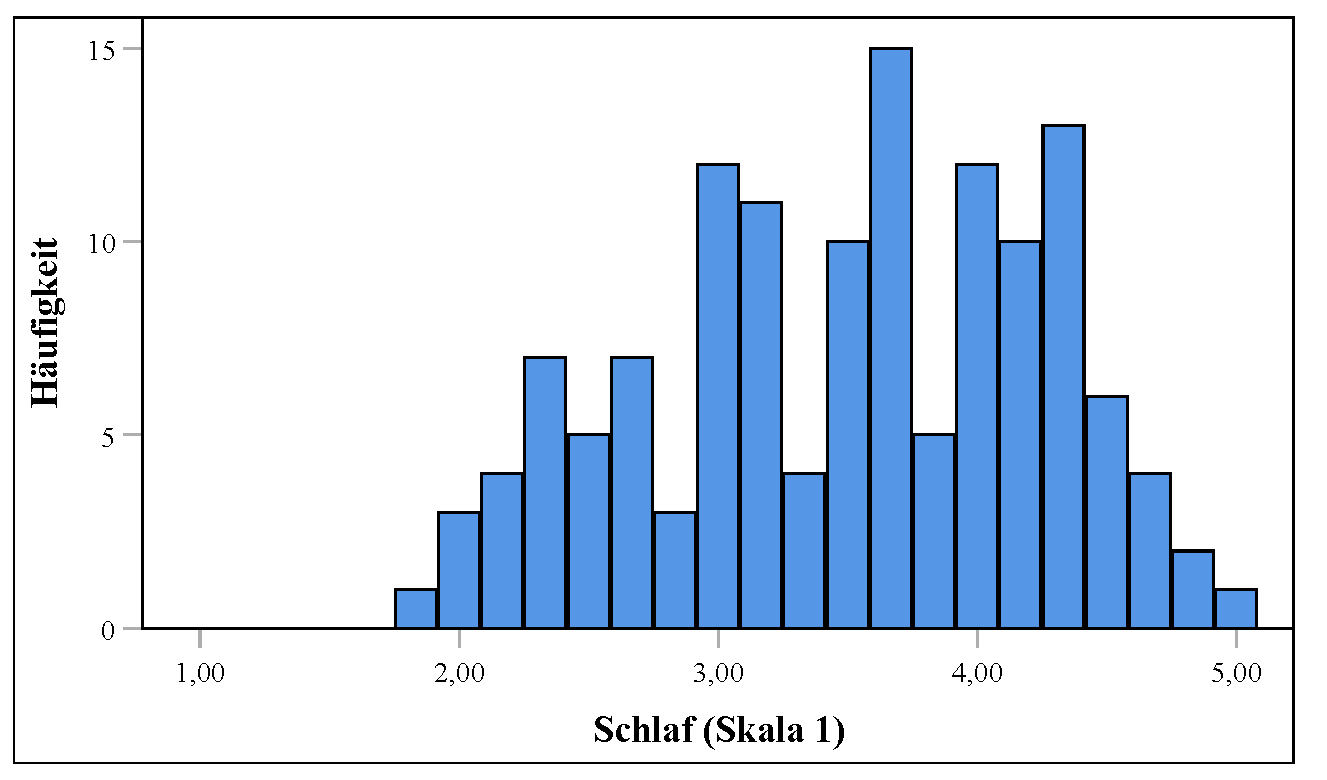
\includegraphics[width=0.8\linewidth]{Histogramm Skala Schlaf.pdf}
        \caption[Histogramm für die Skala Schlaf]{Histogramm für die Skala Schlaf. 
        Codierung: 1.00 = stimme nicht zu ... 5.00~=~stimme vollständig zu. $N = 135$. 
        $M = 3.50$, $SD = 0.76$, $Skewness = -0.25$, $Kurtosis = 0.86$, 
        Cronbachs-\textalpha \ = .72.}
        \label{Histogramm Skala Schlaf}
\end{figure}

Die in dem Histogramm in Abbildung~\ref{Histogramm Skala Ernährung} erkennbare 
Häufigkeitsverteilung ist leicht linksschief (\textit{Skewness} = -0.27) bei einer 
spitzgipfligen Wölbung ($Kurtosis~=~0.65$) und zeigt eine statistisch signifikante 
Abweichung von der Normalverteilung (K-S-Anpassungstest: $p = .008$). Die Mehrheit 
der Befragten berichtet im Durchschnitt somit eher teilweise den Items der 
Ernährungs-Skala zuzustimmen.
\input{Histogramm Skala 2 Ernährung.tex}
\chapter{Diskussion}   \label{ch_4}
Interpretation der Ergebnisse und Reflexion der Arbeit

\section{Zitationsbeispiele}

\textbf{Werk einer Person:} sieht dann im Text so aus. \textcite{Hussy2010} und in 
der Klamer immer so \parencite{Hussy2010}.

\textbf{Körperschaftsautoren:} Beim ersten Auftreten sieht \textcite{6.13t} so aus.
Und in der Klammer sieht eine Körperschaft so aus: \parencite{6.13p}. Bei einer 
wiederholten Erwähnung sieht es dann jeweils so aus: \textcite{6.13t} im Text und 
\parencite{6.13p} in der Klammer.


\subsection{Werk von zwei oder mehr Personen}
\textbf{Werk von zwei Autoren:} Innerhalb des Textes wird die Quelle immer so
verfasst: \textcite{Amelang2006}. In der Klammer so: \parencite{Amelang2006}.

\textbf{Werk von mehr als zwei aber weniger als sechs Autoren:} Das ist der Beginn 
für die erste Erwähnung von vier Autoren, um sie später nochmal zu erwähnen 
\textcite{b0424f3eebf64b03a01a8841d7e3bf8d}. Das hier ist die Art und Weise in 
der Klammer \parencite{b0424f3eebf64b03a01a8841d7e3bf8d}. Und hier werden sie 
wieder erwähntv\textcite{b0424f3eebf64b03a01a8841d7e3bf8d}.

\textbf{Werk von sechs oder mehr Autoren aber unter acht:} So sieht es aus, wenn
sechs Autoren erwähnt werden \textcite{doi:10.1026/1616-3443/a000099}. In der
Klammer steht es wie folgt \parencite{doi:10.1026/1616-3443/a000099}.

\textbf{Werk von mindestens acht Autoren:} Hier werden im Literaturverzeichns nur
die ersten sechs Autoren genannt werden, gefolgt von drei Auslassungspunkten
und am Ende noch der letzte Name. So sieht \textcite{ao1} im Text aus. Und in 
der Klamer dann so: \parencite{ao1}.

\textbf{Werk von einer Person mit zwei Nachnamen:} Etwas gesagt von 
\textcite{AQUINOJARQUIN2021}. Und dann zitieren wir ihn nochmal,aber dieses mal in 
Klammern \parencite{AQUINOJARQUIN2021}.

\subsection{Blockzitat}
\noindent Ein Blockzitat ist ein wörtliches Zitat ab 40 Wörtern.
\begin{Blockzitat}
    CRISPR–Cas systems are recently discovered, RNA-based immune systems that 
    control invasions of viruses and plasmids in archaea and bacteria. Prokaryotes 
    with CRISPR–Cas immune systems capture short invader sequences within the 
    CRISPR loci in their genomes, and small RNAs produced from the CRISPR loci 
    (CRISPR (cr)RNAs) guide Cas proteins to recognize and degrade (or otherwise 
    silence) the invading nucleic acids. There are multiple variations of the 
    pathway found among prokaryotes, each mediated by largely distinct components 
    and mechanisms that we are only beginning to delineate. Here we will review our 
    current understanding of the remarkable CRISPR–Cas pathways with particular 
    attention to studies relevant to systems found in the archaea. 
    \parencite{TERNS2011321}
\end{Blockzitat}


\printbibliography[heading=bibintoc,title={Literaturverzeichnis}]
%%%%%%%%% wenn mehrere Anhänge vorhanden %%%%%%%%%
\begin{appendices}
    \chapter{Boxplot Deutscher Aggressionsfragebogen}            \label{Boxplot_AggroFB}
    %\addcontentsline{toc}{chapter}{A}
    \noindent \textit{Boxplot zur Erfassung der Ausreißer des Deutschen Aggressionsfragebogens}

    \begin{figure}[htb!]
        \centering
            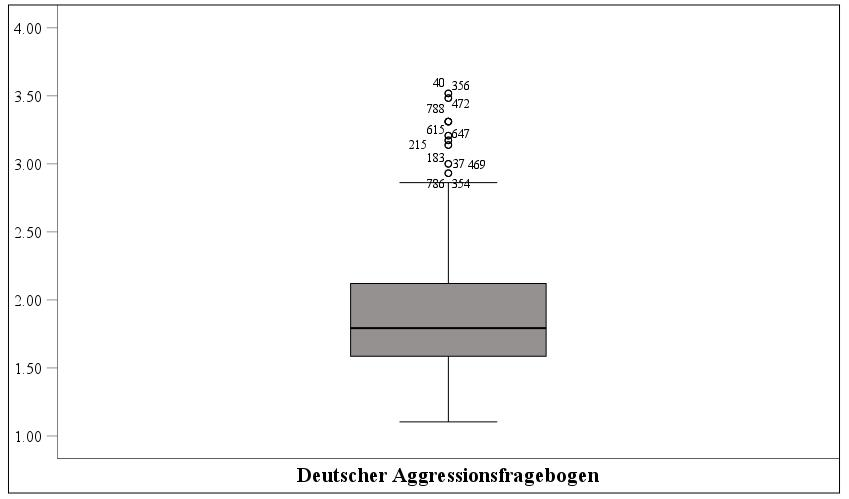
\includegraphics[width=\textwidth]{Boxplot AggroFB.jpg}
            %\caption[Linearer Zusammenhang des Deutschen Aggressionsfragebogens und des DVMAS]{Linearer Zusammenhang des Deutschen Aggressionsfragebogens und des DVMAS}

    \end{figure}
    
    

    %%%%%%%%%%%%%%%%%%%%%%%%%%%%%%%%%%%%%%%%%%%%

    \chapter{Boxplot DVMAS}            \label{Boxplot_DVMAS}
    %\addcontentsline{toc}{chapter}{B}
    \noindent \textit{Boxplot zur Erfassung der Ausreißer des DVMAS}

    \begin{figure}[htb!]
        \centering
            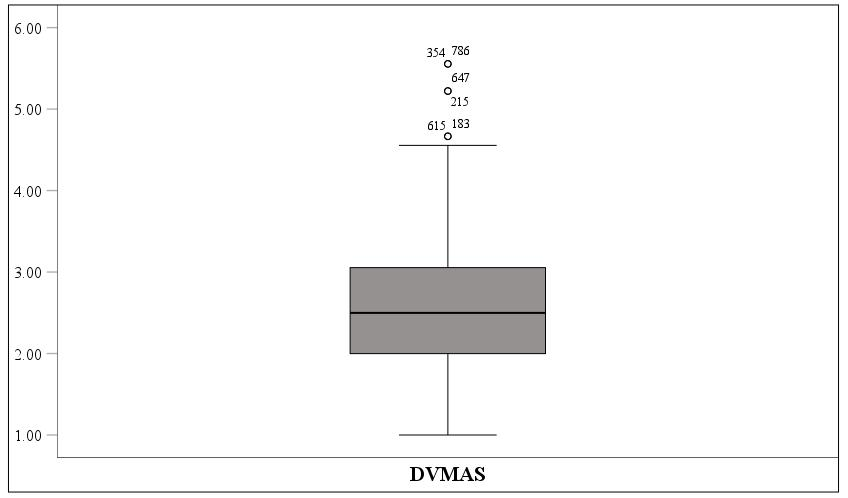
\includegraphics[width=\textwidth]{Boxplot DVMAS.jpg}
            %\caption[Linearer Zusammenhang des Deutschen Aggressionsfragebogens und des DVMAS]{Linearer Zusammenhang des Deutschen Aggressionsfragebogens und des DVMAS}

    \end{figure}
    
    

%%%%%%%%%%%%%%%%%%%%%%%%%%%%%%%%%%%%%%%%%%%%

\chapter{Linearität Deutscher Aggressionsfragebogen und DVMAS} \label{Linearitat_AggroFB_DVMAS}
%\addcontentsline{toc}{chapter}{C}
\noindent \textit{Linearer Zusammenhang des Deutschen Aggressionsfragebogens und des DVMAS}

\begin{figure}[htb!]
    \centering
        \includegraphics[width=\textwidth]{Linearität AggroFB-DVMAS.jpg}
        %\caption[Linearer Zusammenhang des Deutschen Aggressionsfragebogens und des DVMAS]{Linearer Zusammenhang des Deutschen Aggressionsfragebogens und des DVMAS}
        
\end{figure}
    
    

%%%%%%%%%%%%%%%%%%%%%%%%%%%%%%%%%%%%%%%%%%%%

    \chapter{Boxplot Aggression$-$Subskala physische Aggression}            \label{Boxplot_phAggro}
    %\addcontentsline{toc}{chapter}{D}
    \noindent \textit{Boxplot zur Erfassung der Ausreißer der Aggression$-$Subskala physische Aggression}

    \begin{figure}[htb!]
        \centering
            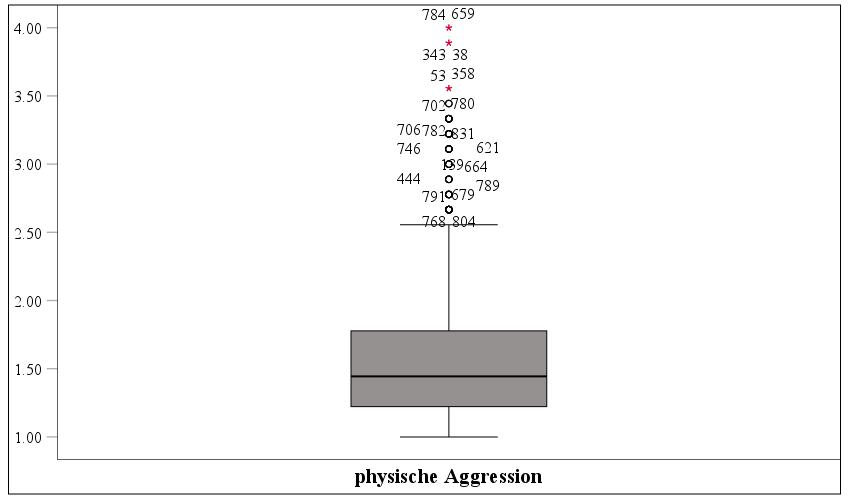
\includegraphics[width=\textwidth]{Boxplot ph_aggro.jpg}
            %\caption[Linearer Zusammenhang des Deutschen Aggressionsfragebogens und des DVMAS]{Linearer Zusammenhang des Deutschen Aggressionsfragebogens und des DVMAS}

    \end{figure}
    
    

%%%%%%%%%%%%%%%%%%%%%%%%%%%%%%%%%%%%%%%%%%%%

    \chapter{Online$-$Fragebogen}  \label{Fragebogen}
    %\addcontentsline{toc}{chapter}{E}
    \noindent \textit{Bildaufnahmen des Online$-$Fragbogens}

    \begin{figure}[htb!]
        \centering
            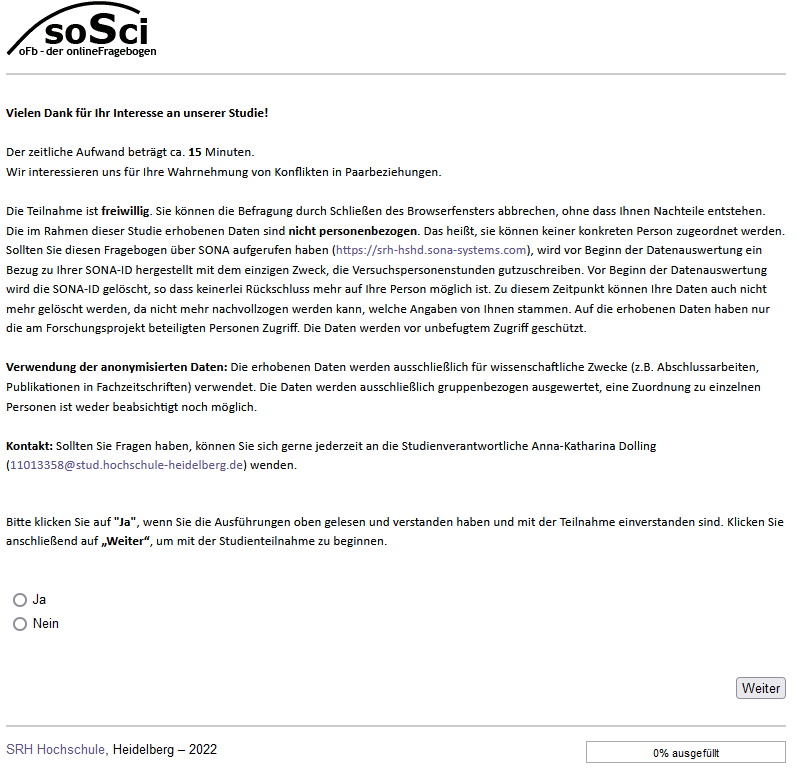
\includegraphics[width=\textwidth]{Seite 1.png}
            \caption[]{Seite 1 des Online$-$Fragebogens}
    \end{figure}

    \newpage
    \begin{figure}[htb!]
        \centering
            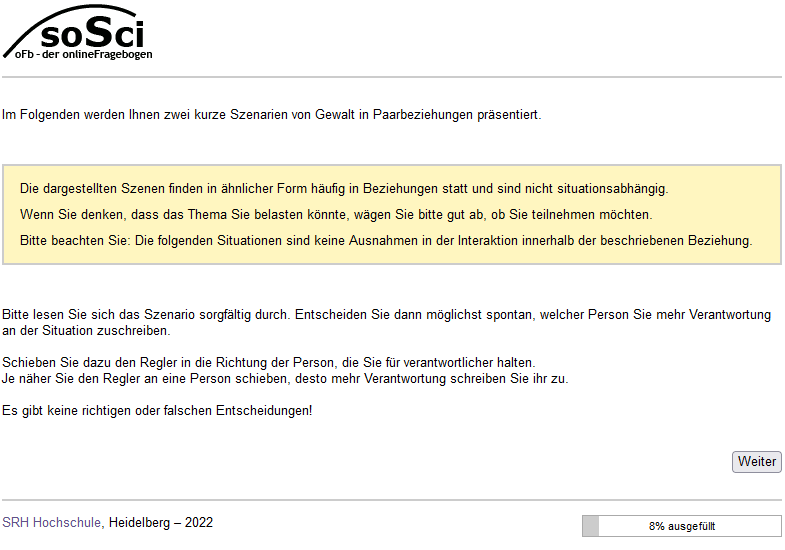
\includegraphics[width=\textwidth]{Seite 2.png}
            \caption[]{Seite 2 des Online$-$Fragebogens}
    \end{figure}

    \begin{figure}[htb!]
        \centering
            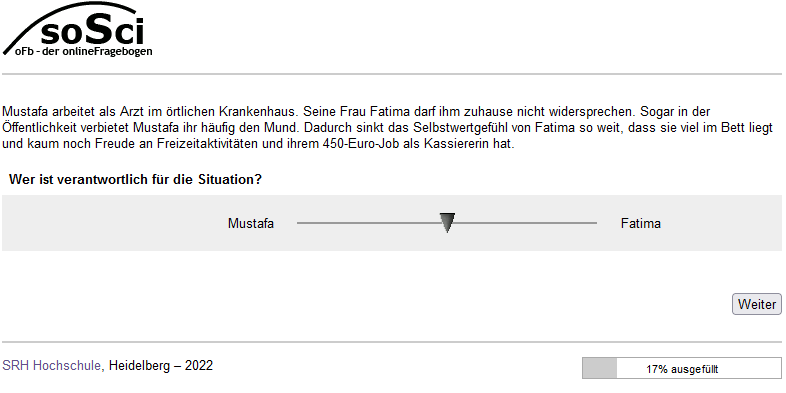
\includegraphics[width=\textwidth]{Seite 3.png}
            \caption[]{Seite 3 des Online$-$Fragebogens}
    \end{figure}
    
    \newpage
    \begin{figure}[htb!]
        \centering
            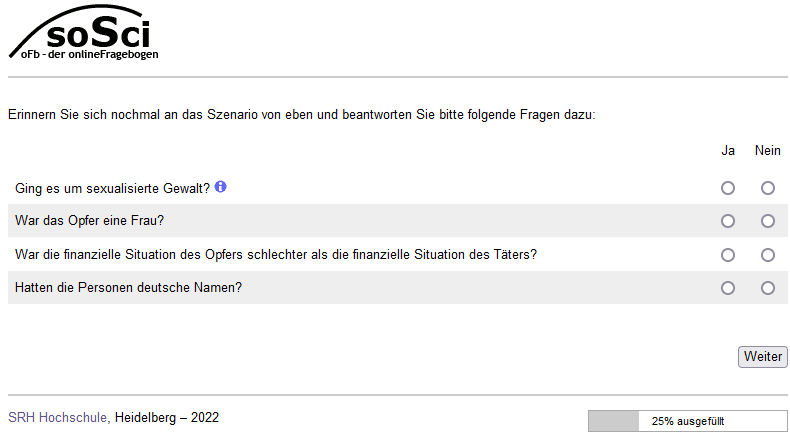
\includegraphics[width=\textwidth]{Seite 4.png}
            \caption[]{Seite 4 des Online$-$Fragebogens}
    \end{figure}
    
    \begin{figure}[htb!]
        \centering
            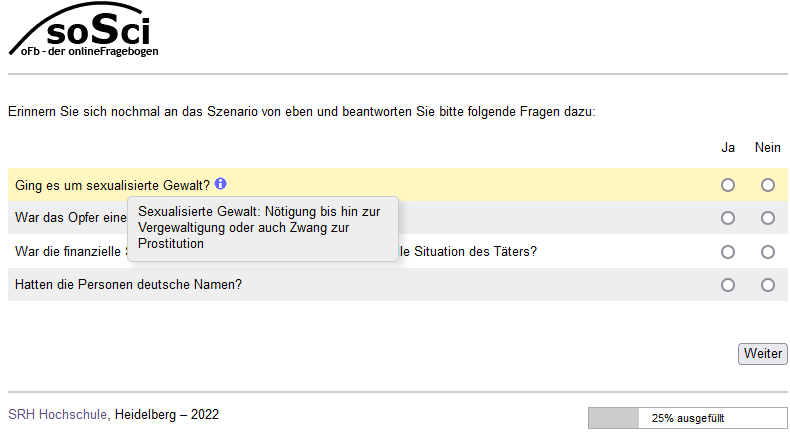
\includegraphics[width=\textwidth]{Seite 4 mit Infobox.png}
            \caption[]{Seite 4 des Online$-$Fragebogens mit Infobox}
    \end{figure}
    
    \newpage
    \begin{figure}[htb!]
        \centering
            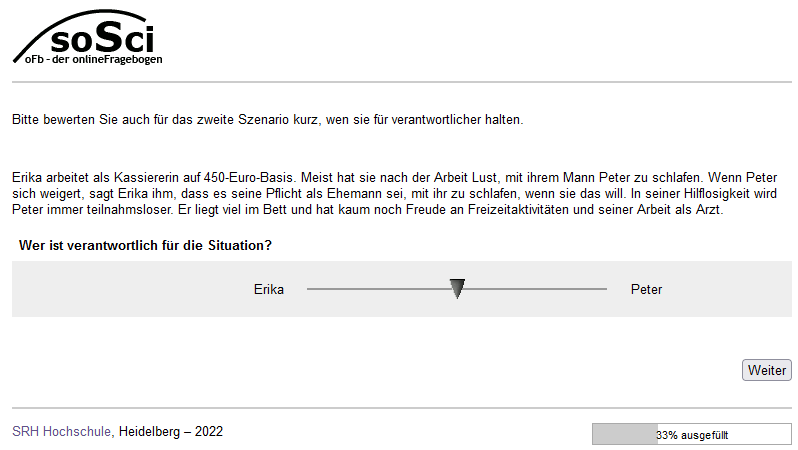
\includegraphics[width=\textwidth]{Seite 5.png}
            \caption[]{Seite 5 des Online$-$Fragebogens}
    \end{figure}
    
    \begin{figure}[htb!]
        \centering
            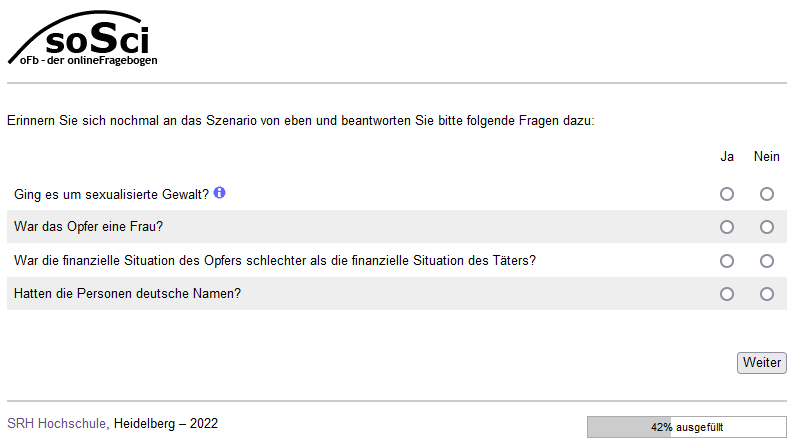
\includegraphics[width=\textwidth]{Seite 6.png}
            \caption[]{Seite 6 des Online$-$Fragebogens}
    \end{figure}
    
    \newpage
    \begin{figure}[htb!]
        \centering
            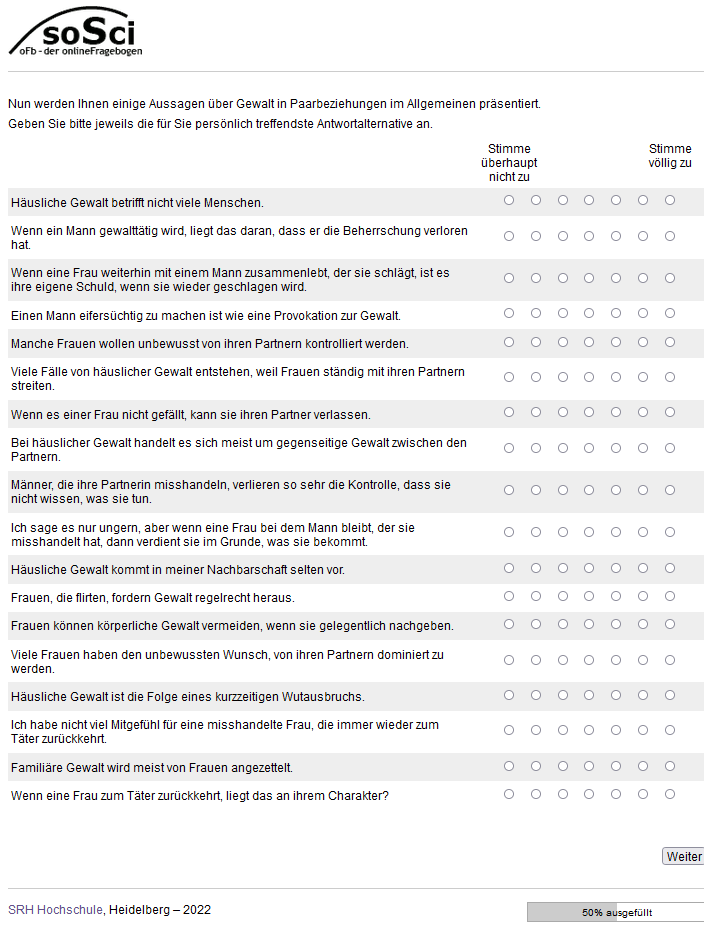
\includegraphics[width=\textwidth]{Seite 7.png}
            \caption[]{Seite 7 des Online$-$Fragebogens (deutsche Übersetzung des englischen DVMAS nach \textcite{Peters2003})}
    \end{figure}
    
    \newpage
    \begin{figure}[htb!]
        \centering
            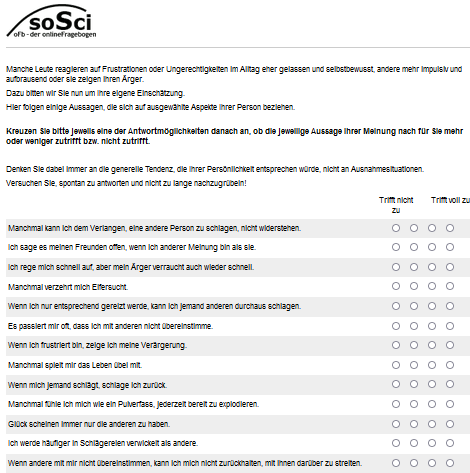
\includegraphics[width=\textwidth]{Seite 8_1.png}
            \caption[]{Erste Hälfte von Seite 8 des Online$-$Fragebogens des Deutschen Aggressionsfragebogens \parencite{Aggressionsfragebogen}}
    \end{figure}
    
    \newpage
    \begin{figure}[htb!]
        \centering
            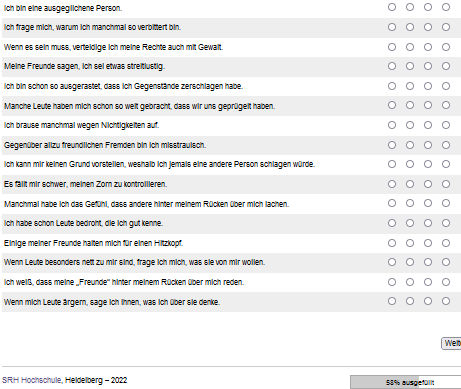
\includegraphics[width=\textwidth]{Seite 8_2.png}
            \caption[]{Zweite Hälfte von Seite 8 des Online$-$Fragebogens des Deutschen Aggressionsfragebogens \parencite{Aggressionsfragebogen}}
    \end{figure}
    
    \newpage
    \begin{figure}[htb!]
        \centering
            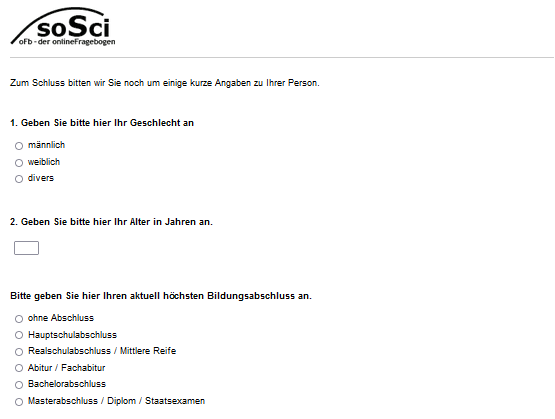
\includegraphics[width=\textwidth]{Seite 9_1.png}
            \caption[]{Erste Hälfte von Seite 9 des Online$-$Fragebogens}
    \end{figure}
    
    \newpage
    \begin{figure}[htb!]
        \centering
            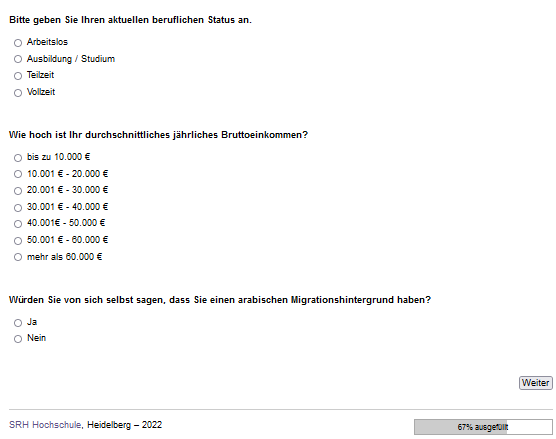
\includegraphics[width=\textwidth]{Seite 9_2.png}
            \caption[]{Zweite Hälfte von Seite 9 des Online$-$Fragebogens}
    \end{figure}
    
    \begin{figure}[htb!]
        \centering
            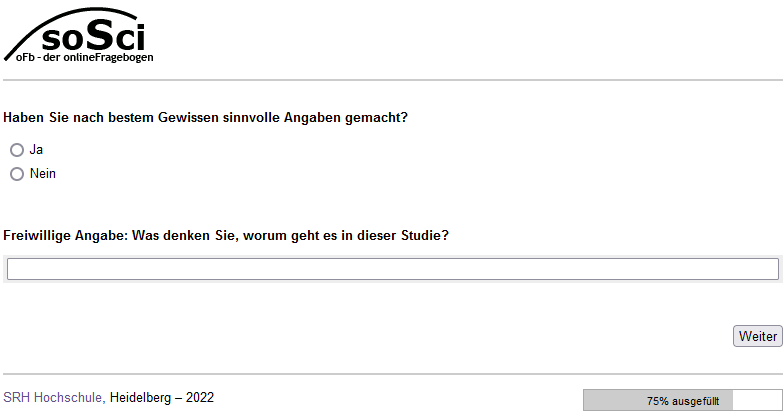
\includegraphics[width=\textwidth]{Seite 10.png}
            \caption[]{Seite 10 des Online$-$Fragebogens}
    \end{figure}
    
    \newpage
    \begin{figure}[htb!]
        \centering
            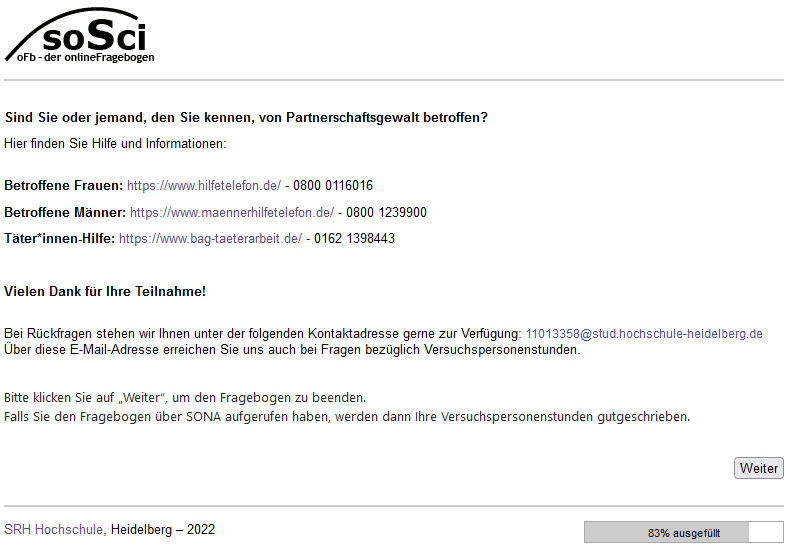
\includegraphics[width=\textwidth]{Seite 11.png}
            \caption[]{Seite 11 des Online$-$Fragebogens}
    \end{figure}
    
    \begin{figure}[htb!]
        \centering
            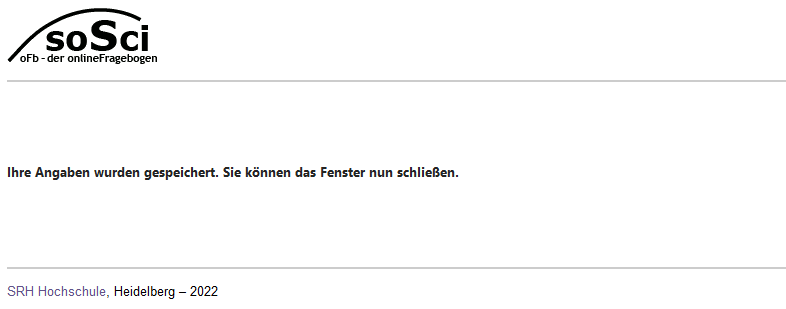
\includegraphics[width=\textwidth]{Seite 12.png}
            \caption[]{Seite 12 des Online$-$Fragebogens}
    \end{figure}


    
    

%%%%%%%%%%%%%%%%%%%%%%%%%%%%%%%%%%%%%%%%%%%%
\end{appendices}







%%%%%%%%% wenn mehrere Anhänge vorhanden %%%%%%%%%



%%%%%%%%% wenn nur 1 Anhang vorhanden %%%%%%%%%
%\chapter*{Anhang}
%\addcontentsline{toc}{chapter}{Anhang}
%\noindent \textit{Titel des Anhangs}

%Inhalt
%%%%%%%%% wenn nur 1 Anhang vorhanden %%%%%%%%%
\newpage
\fontsize{18pt}{0pt}\textbf{Ehrenwörtliche Erklärung}
\parskip=32pt

\noindent Gemäß Studien- und Prüfungsordnung erklären wir, dass wir diese schriftliche 
Hausarbeit selbstständig angefertigt und wörtliche und sinngemäße Zitate 
kenntlich gemacht haben. Mit der Überprüfung auf etwaige Übereinstimmungen mit 
fremden Quellen mit Hilfe von Anti- Plagiatssoftware sind wir einverstanden. 
Wir erklären außerdem, dass diese Arbeit nicht im Rahmen eines anderen 
Prüfungsverfahrens bereits vorgelegt wurde. 
\parskip=32pt

\noindent Heidelberg, den \today
\parskip=32pt

\noindent Unterschriften:

[Unterschrift 1]

[Unterschrift 2]
\end{document}
